%%%%%%%%%%%%%%%%%%%%%%%%%%%%%%%%%%%%
\chapter{Introduction}
\label{chap:Introduction}
%%%%%%%%%%%%%%%%%%%%%%%%%%%%%%%%%%%%

\comment{

The introduction should provide:
\begin{itemize}
    \item A clear explanation of the problem that you tackle
    \item Motivation why this is interesting and worth investigating
\end{itemize}

To improve communication, it is also recommended that you concisely state the aims and objectives of your project.  As part of the introduction, these can be generally stated and not require specialist knowledge.  Use the next chapter "Literature Review" to provide specialist knowledge for the reader.
\begin{enumerate}
    \item \textbf{Aims:} The aims of a project are \emph{what you hope to learn}.
        \begin{enumerate}
        \item "To understand why X varies with Y..."
        \item "To evaluate [technology] when exposed to unexpected conditions so that..."
        \item "To increase understanding of ..."
        \item \emph{etc...}
        \end{enumerate}
    \item \textbf{Objectives:} The objectives are \emph{the elements which are necessary to conduct the project}.
        \begin{enumerate}
            \item "To properly design an experiment methodology to mitigate...."
            \item "To construct a robotic system including ... to collect meaningful data."
            \item "A complete analysis of ... must be conducted prior to the full system evaluation in order to..."
            \item \emph{etc...}
        \end{enumerate}
\end{enumerate}

You can then repeat and address these explicitly in your Conclusion when evaluating the success and challenges of your project. 

}

\section{Aims}

Based on the self-organised channel resource allocation principle of the STDMA
(Self-organised Time Division Multiple Access) \cite{STDMA} communication protocol, develop
a method for agents to achieve collision-free moving on a 2D plane, make it self-organised,
decentralised and scalable.

% 注意,这里后面可以用一个itemize将算法所需要达到的性能展开说


\section{Objectives}

% 注:objectives里面后续可以加上为什么要这么做,譬如:为了观察。。。,必须构建一个。。。

\begin{itemize}
    \item  Develop a multi-agent communication scenario with STDMA in ROS2. In this 
    scenario, multiple identical agents will share the same channel and all agents
    have both receiving and transmitting capabilities. The goal is to enable agents to
    autonomously organise/join the communication process after start up. 
    \item On the basis above, a grid world is implemented: a 2D map composed of grids, 
    each grid represent a part of space. Agents could move from one grid to another in the map.
    \item \dots
\end{itemize}

\section{Motivation}

The motivation of this project is to answer a question inspired by \cite{Paper_From_Supervisor}, which is:

\begin{quote}
    \textbf{What will happen if use STDMA for 2D resource sharing?}
\end{quote}

The detailed explanation of the motivation is as follows.

\subsection{Why STDMA?}

\label{sec:Why STDMA?}

\textbf{What is STDMA?} The \textit{Self-organised Time Divided Multi Access} (STDMA)
 is a channel access technique for communication. 
 It is based on a set of policies dictating how agents ought to apply for
  slots in repeating frames. 
  In short, STDMA is a protocol that allows agents to autonomously
   share 1D resources (time) among themselves.

   % 记得加上:详细的解释位于文献综述部分

The reason for using STDMA is its \textbf{characteristics}:

\begin{enumerate}
    \item \textbf{Deterministic}: Agents arrange their data transmission based on a determined timetable.
    \item \textbf{Decentralised}: Agents listen to the channel first, then find free slots in the timetable for themselves to use.
\end{enumerate}

These characteristics could be useful for multiple agents to achieve collision-free (use free slots only),
 self-organised (find slots on its own) resource sharing.

There are also two \textbf{reasons that making this challenging}: 

\begin{enumerate}
    \item \textbf{Purpose difference}: In the original STDMA, an agent only needs to find one unused slot
    in the repeating frame (which is generally of a fixed length chosen manually) and maintain ownership of that slot,
    which means agents don't need to move from one slot to another slot, i.e., don't have destination in the channel allocation timetable. 
    But that's different for 2D space moving, where agents have their destinations and need to move grid by grid to reach their goals.
    % 这里可以补一句话,关于如果直接使用在2D中会导致的可能结果。来具体说明这种用途的不同到底会造成什么结果
    \item \textbf{Complexity difference}: Channel sharing only requires randomly selecting one slot from the known free slots, while space sharing in
     a 2D plane requires the agent to find a path that doesn't collide with other agents, and the possibility space for the path could be enormous
      (map size $\times$ predicting horizon), but the processing time available to the agent is limited
       (must broadcast its presence at regular intervals so that other agents can be aware of its plans and thus avoid collisions).
\end{enumerate}


These characteristics and challenges make this project interesting and worthy of research.


\subsection{Why 2D plane path planning?}

2D plane path planning is a name for better understanding and is not the accurate name for this problem.
This problem is acturally a \textbf{\textit{Multi-Agent Path Finding} (MAPF)} problem \cite{MAPF_Explain1, MAPF_Explain2}.

Here, the term "finding" could be somewhat confusing. 
In fact, he MAPF problem combines both \textbf{collision-free movement} of multiple agents and 
\textbf{path efficiency optimising}.

Overall, the problem of \textit{Multi-Agent Path Finding} (MAPF) concerns \textbf{the movement of multiple agents in a grid world}.

To easily get a better understanding of this problem, please refer to this \href{https://primalgrid.netlify.app/primal}{website}\footnotemark.\footnotetext{https://primalgrid.netlify.app/primal}
The website presents the MAPF problems and their solutions through a simple and engaging animation (estimated time required: 1$\sim$2 min).

% 记得加上:详细描述参看后续Literature review

%\FloatBarrier
\begin{figure}
    \centering
    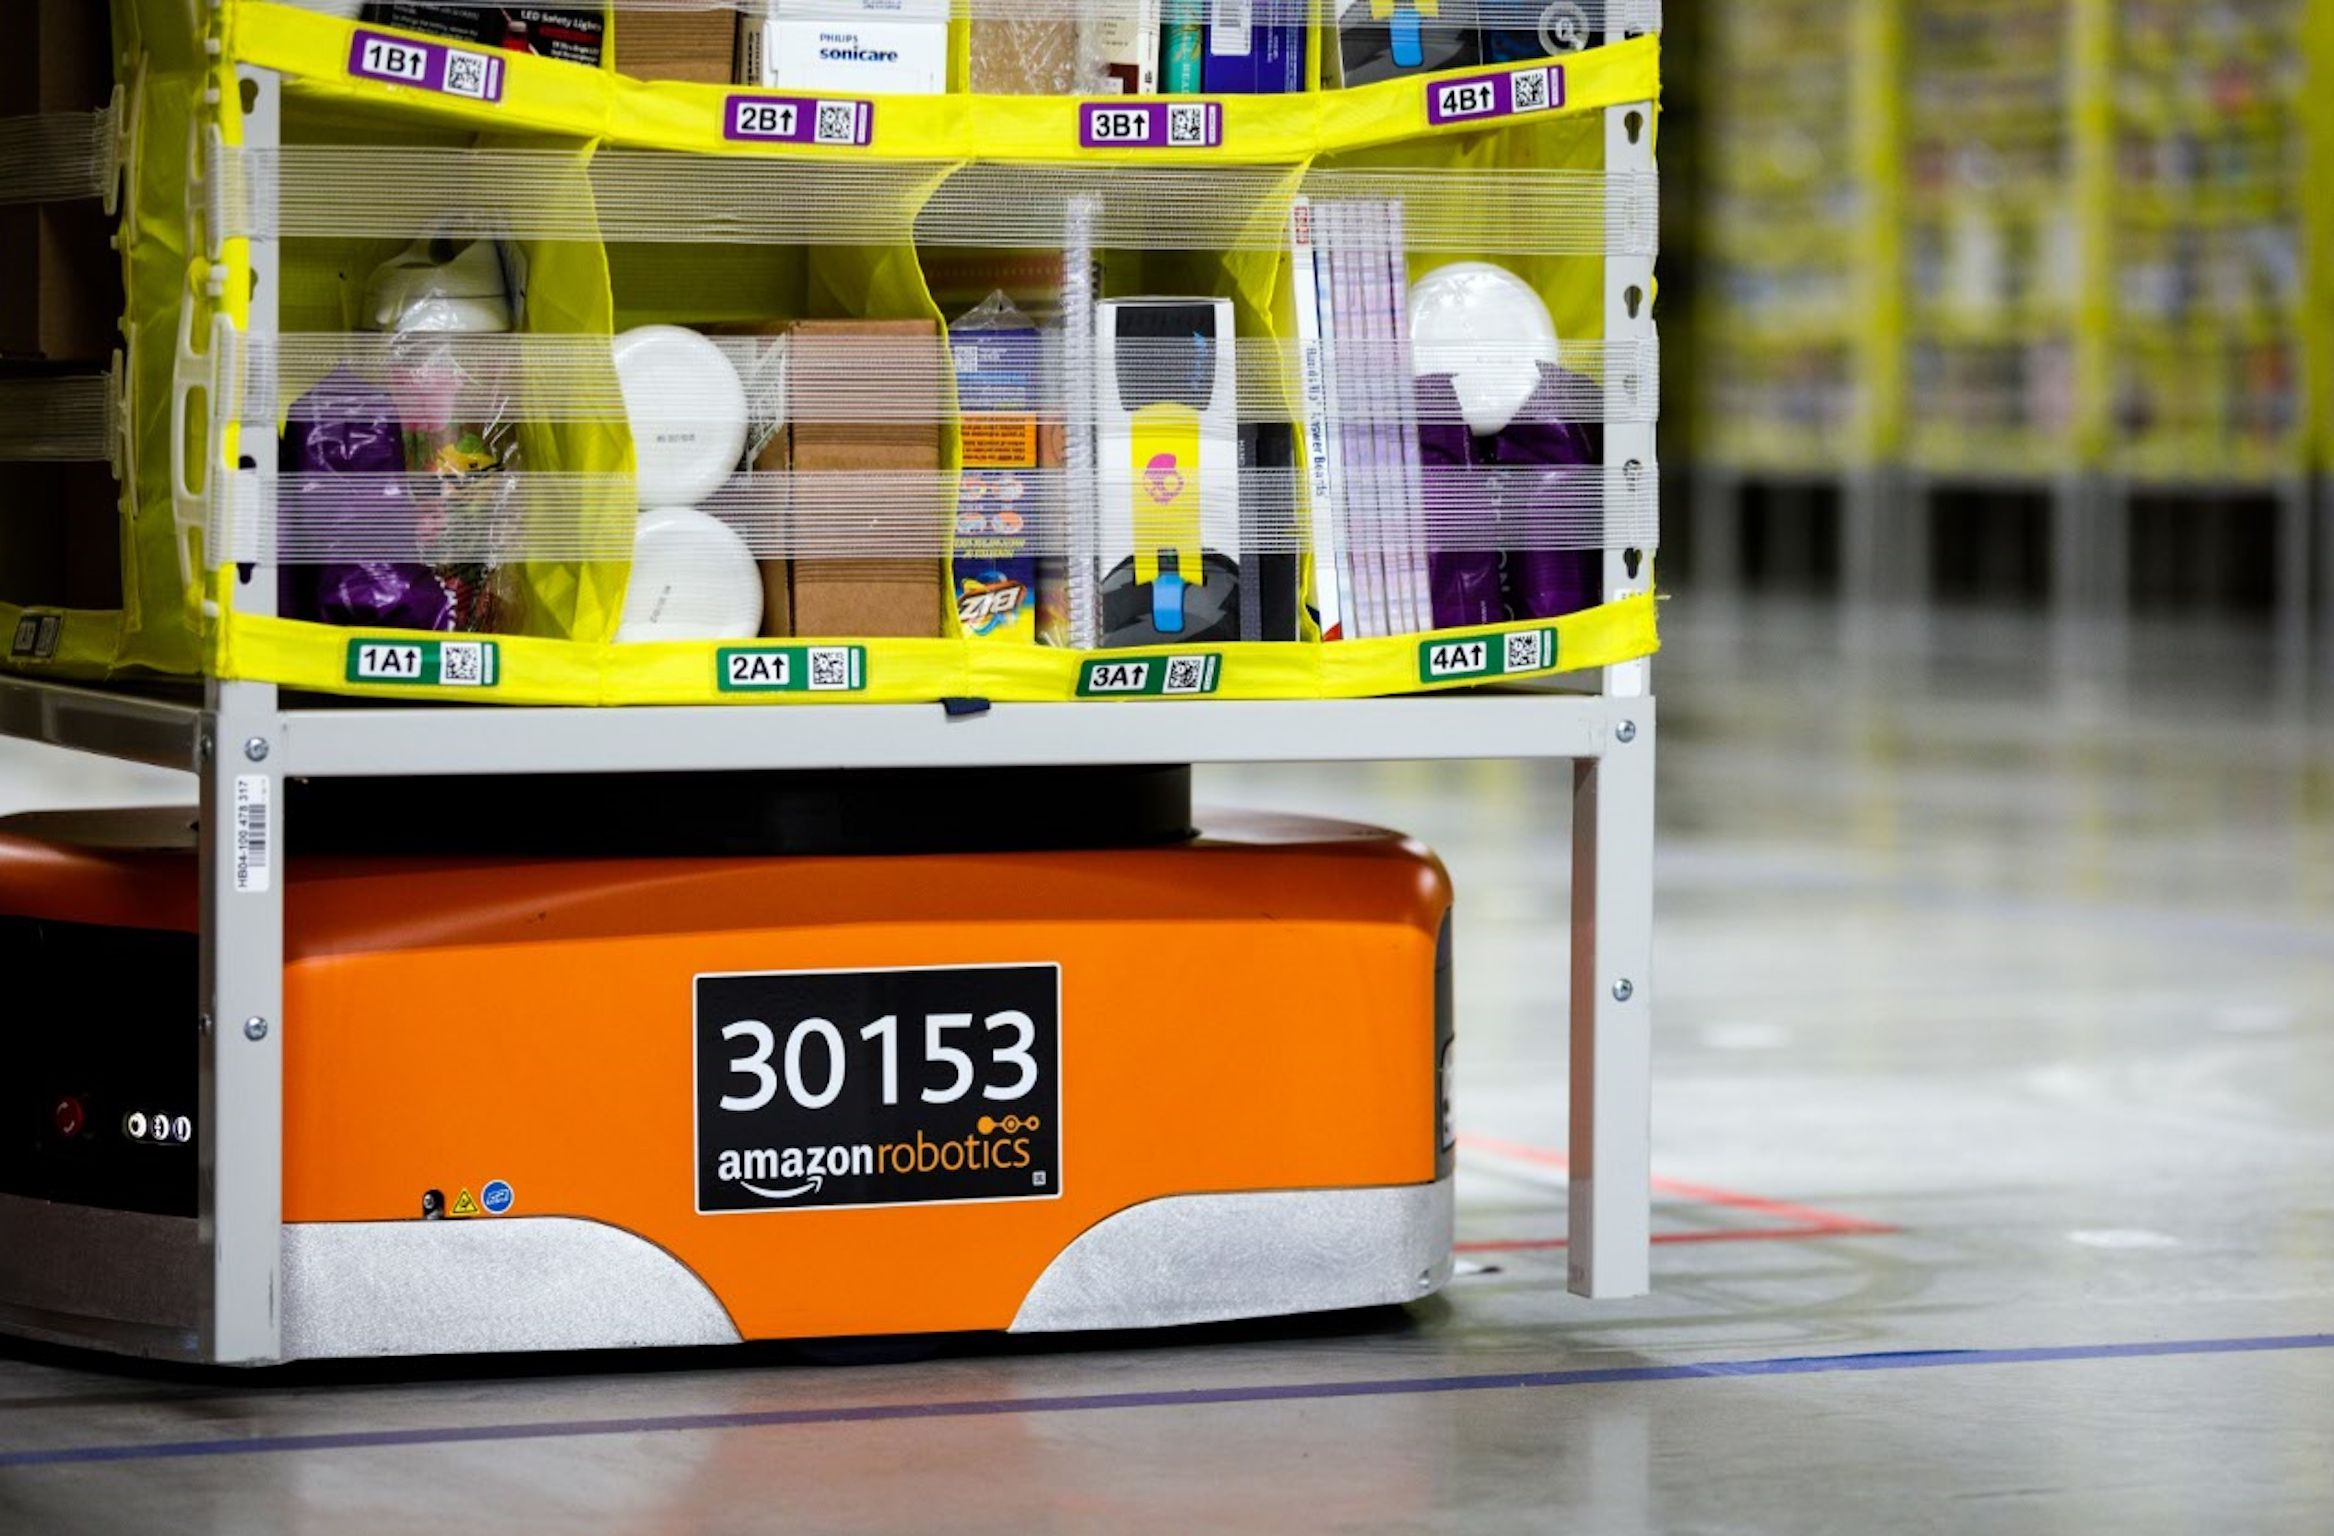
\includegraphics[width=0.6\linewidth]{figures/Amazon_Warehouse.jpeg}
    \caption{Kiva system operating in Amazon warehouse\protect\footnotemark. }
    \label{fig:Amazon Warehouse Robots}
\end{figure}
\footnotetext{https://spectrum.ieee.org/interview-brad-porter-vp-of-robotics-at-amazon}

\textbf{MAPF algorithms have broad prospects for use}.
\begin{itemize}
    \item \textbf{Warehouse Automation}: Pick-pack-and-ship system in warehouse (like Fig \ref{fig:Amazon Warehouse Robots}). Delivering items in sorting station \cite{Warehouse_Automation1,Warehouse_Automation2}.
    \item \textbf{Intersection Management}: Coordinate autonomous vehicle movement through intersections \cite{Intersection_Management}.
    \item \textbf{Robot Fleet}: Automating fleets of autonomous robots like forklift fleets \cite{Fork_Fleet1,Fork_Fleet2}.  
    \item \textbf{Agents in video games and CGIs}: Flock simulating and animating\cite{Flocking_1,Flocking_2}.
    \item \textbf{Swarm Robots}: Controlling self-organised robot swarms\cite{Swarm_Robotics}.
\end{itemize}

In general, the application of this algorithm is very broad. Furthermore, in the context of Industry 4.0 and flexible manufacturing, it has even better prospects for application\cite{Industry_41,Industry_42,Industry_43}, as centralized control is gradually becoming inadequate to meet new production needs.
 